\chapter{Test and Evaluation} \label{sec:tests}

The conceptualization of the tests focused in evaluating how well the solution performs with the constrains made in the hardware and software choices. It aims at testing the \ac{rf} solution performance and validate the platform data flow from tag to client.
The moment the final design of the smart shelf was settled, it was evident that two problems could compromise the performance of the solution: the metal structure of the shelf and the old, not maintained, Fosstrak open-source software.

In this chapter will be presented a few tests designed to hint and show how these problems compromise the solution. Throughout the tests, the tags were attached to empty sleeves and boxes, representing an ideal test environment with no \ac{rf} quality compromising materials~\footnote{It was not possible to attain sleeves with aluminum capsules for testing. They would certainty interfere with the following test results, but not accounted in the work of this dissertation.}.
The reader configuration used for the tests maintains the same power transmission ($30dBm$) and sensibility ($-80dBm$) configurations.

\section{Tag orientation} \label{sec:test1}

Prior to the implementation of the final solution, an \ac{rf} analysis of tag orientation in the shelf was conducted.
The objective was to evaluate the optimal tag orientation in stored products, and provide an idea of system reading performance early in the development.
Tags were tested in tree different orientations, illustrated in figure~\ref{fig:tagorientations}.

\begin{figure}
    \centering
    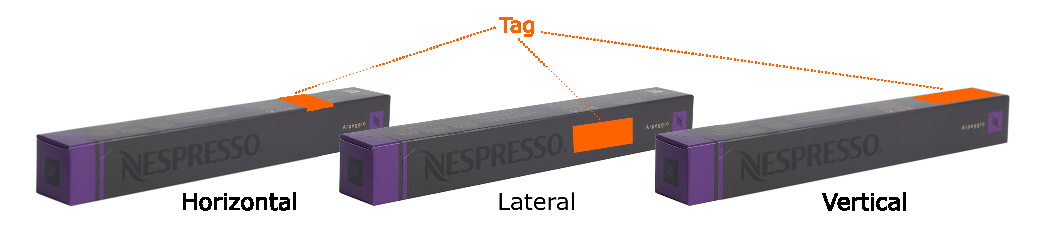
\includegraphics[width=\textwidth]{figs/tests/tag_positions.eps}
    \caption{Tag orientation tested in this dissertation: horizontal, lateral and vertical, respectively}
    \label{fig:tagorientations}
\end{figure}


This test was executed solely on the bottom shelf, since the results could be inferred to the others. The bottom shelf also presented the major apparent challenges: it had to operate in the \emph{near-field} and was too close to the antenna, which could cause miss readings in the outer laterals due to the beam width not being wide enough.

The test was conducted by dividing the bottom shelf into $18$ quadrants ($26.6\times20$cm quadrants) and measure \ac{rssi} values, referent to a single tag, within those quadrants, with a transmission power of $30$dBm and maximum sensitivity of $-80$dBm. The \ac{rssi} results are a mean value calculated from $1000$ values sampled from each quadrant in a uniform motion across the area, repeated in same manner for each quadrant.

The results are shown in figure~\ref{fig:tagorientationsresults} in heatmap plots.
They do not represent the obstructions spread across the shelf. These obstructions prevent tag readings, which were not accounted in this test. Obstructions will be evaluated in the next test.

From the results obtained, there was no clear superior orientation. The circular Keonn Advantenna-p14 in conjunction with the \ac{rf} signal deformations caused by the metal structure, make a good job in providing orientation independence.

\begin{figure}
    \centering
    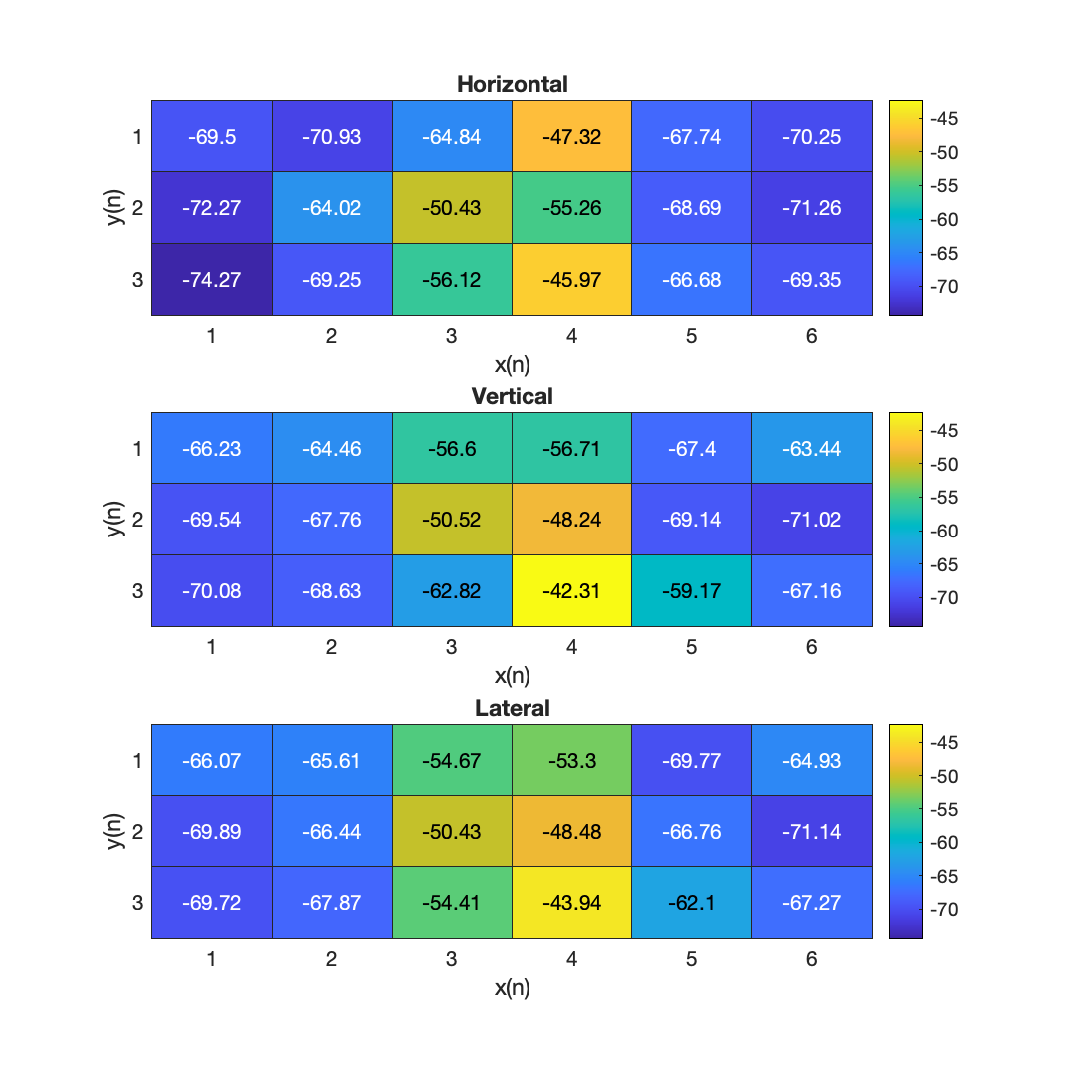
\includegraphics[width=0.7\textwidth]{figs/tests/RSSI_shelve.eps}
    \caption{\ac{rssi} reading results for the different considered tag orientations in dBm}
    \label{fig:tagorientationsresults}
\end{figure}

A few peculiar observations from the tests were observed and are described next:

\begin{itemize}
    \item Horizontal orientated tags have reading problems near the shelf outside metal structure;
    \item Vertical orientated tags, in contrast with horizontal orientated ones, have better reading values near the shelf outside metal structure. They present problems placed on top of the metal bars used to support the shelves.
    \item Lateral orientated tags present reading difficulty when placed on top of the support metal bars and really close to conners.
\end{itemize}

No major benefits were presented by any orientation.
Theoretically, the lateral tag orientation would present most problems, being parallel to the axis of the \acp{emw} propagation.
In order to test the system in the most extreme conditions, the lateral orientation was used for sleeves throughout the dissertation and horizontal orientation for product cases for transport.

\section{Shelf \acs{rf} Survey}

The objective of this test was to study and evaluate the certainty and quality of tag readings, by making an \ac{rf} survey of the shelf, with the lateral tag orientation defined previously.
It aims at evaluating the \ac{rf} obstructions present in the solution, which were not considered in the first test.
The results should offer a good representation of the \ac{rf} environment in the shelf and what it could be expected from tag readings in certain locations. 
From the previous test, it was observed that the \ac{rssi} does not change in time when a single tag is placed in one specific location, allowing the sampling of a single \ac{rssi} value per location. 

The test consisted, once again, in dividing the shelves into quadrants and measure \ac{rssi} values within those quadrants. This time, each shelf was divided in $140$ quadrants ($20\times7$ grid, $8\times8.6$cm quadrants) to have a better perspective of \ac{rf} obstructions. Measurements were also taken in between shelves. The transmission power and sensitivity were maintained from the previous test.
The results can be seen in figure~\ref{fig:rfsurvey}.

\begin{figure}
    \centering
    \includegraphics[width=0.7\linewidth]{./figs/tests/rfsurvey-old.eps}
    \caption{Shelf \acs{rf} survey showing the \ac{rssi} values within the $20\times7$ grid}
    \label{fig:rfsurvey}
\end{figure}

It is possible to observe the obstructions caused from the metal bars used to support the middle of each shelf. The surrounding metal structure does not seem to interfere significantly to the point of tag blocking readings. We can also observe poor \ac{rssi} values near the first shelf, as observed in previous test with lateral orientated tags.
To have a better perspective on obstruction points across the shelves, in relation to the support metal bars and antenna placement, a graph with those illustrated is shown in figure~\ref{fig:shelveobstructions}. 

\begin{figure}
    \centering
    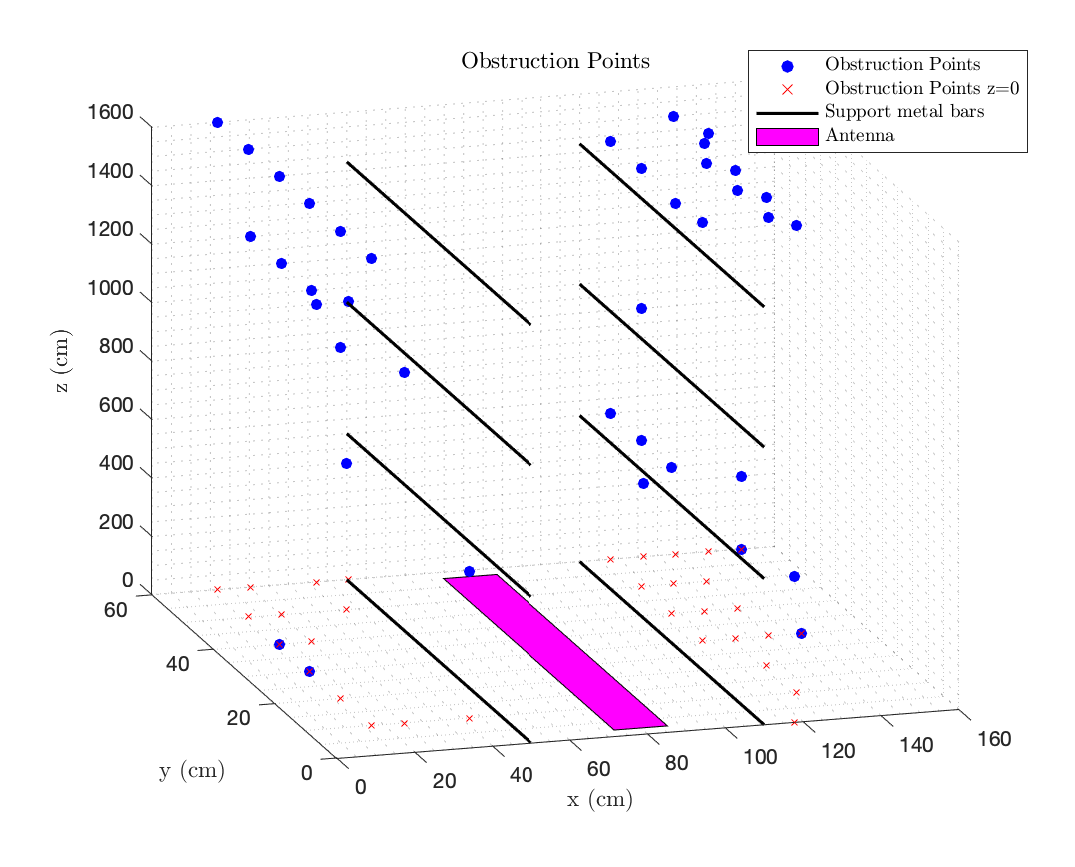
\includegraphics[width=0.7\textwidth]{figs/tests/obstructions.eps}
    \caption{\acs{rf} survey obstructions points shown in conjunction with support metal bars and antenna placement}
    \label{fig:shelveobstructions}
\end{figure}

\section{Singulation stress test}

This test aimed at complementing the observations from previous test by evaluating how the obstructions affect readings of a group of tags placed on top \ac{rf} ``blind'' quadrants.
The test method consisted of selecting locations were obstructions were prevalent and for each one, at a time, place boxes full of sleeves in those positions to evaluate for miss readings.

From this test it was possible to retrieve some interesting observations. 
As expected, \ac{rf} obstructions cause miss readings, but the phenomenon is not as linear as the previous tests, which used a single tag. 
Some obstruction locations did not present miss readings. In those locations, when a sleeve was removed from the case for transport, a tag would miss read, as illustrated in figure~\ref{fig:missreading}. The ``disappearing'' tag could be right next to the removed one or in other box, not being evident the obstruction phenomenon happening.
The phenomenon can be linked to:

\begin{itemize}
    \item \ac{rf} obstructions resulting from the presence of \ac{rf}-opaque or \ac{rf}-absorbent objects which block and absorb \ac{rf} waves respectively~\cite{lahiriRFIDSourcebook2005};
    \item ``Re-radiating'' phenomenon due to the \emph{near-field} Fresnel region reacting with the metal structure and the tags antennas themselves~\cite{ElectromagneticRadiationField};
    \item Tag-to-tag interference.
\end{itemize}

\begin{figure}
    \centering
    \includegraphics[width=0.4\textwidth]{figs/tests/missread.eps}
    \caption{Non linear obstruction phenomenon illustrating miss readings caused by the removal of a tagged sleeve}
    \label{fig:missreading}
\end{figure}

More research and tests have to be performed in order to confirm these hypotheses.
To complement the observations in these tests, a few metal objects were placed on the shelf, namely an aluminum notebook computer, an aluminum window frame, and a steel oil heater placed near the shelf.
The aluminum notebook and window placed in different locations, would interfere with the tag readings. The steel oil heater placed leaning on the shelf did not seem to interfere in any way, indicating a good and confined shelf \ac{rf} radiation.

\section{Operational test}

For the final test, the objective is to validate the platform operation.
The test consisted of making inventory changes and validating through the web management application and database entries if the data is in accordance with those changes, namely if tags added and removed are adequately identified.

The platform was able to adequately read the inventory changes, publish them to the \ac{epcis} repository and be visualized in the web management application.

\subsection{Problems}

Some problems of the software platform were already hinted throughout this dissertation, namely in section~\ref{sec:softwareplatformoptions}.
The Fosstrak software components used in this dissertation are not maintained. The problems caused by bugs, confusion in outdated documentation and runtime errors were the issues that took most working hours in this dissertation, many which could not be solved.
Modern Java and Tomcat versions created breaking changes in the code, which forced the use of old versions. 
These old versions also did not solve all the problems, but reduced the amount of bugs to a point where the platform was working. A few major problems presented in the final platform solution will be described next.

Starting with the \ac{fc} middleware, it presents multiple problems. 
The web-based client is broken. The static logical reader definitions are broken.
The standalone client works, but when registering \acp{lrspec} and \acp{ecspec}, most of the times, causes the server to break due to concurrent modification thread errors.

The capture application also presents a few problems.
The connection between the \ac{ale} interface of the capture application and the middleware seems to have some issues. Using the middleware log information, it is possible to verify that the middleware processes the reports delivered by the reader, but they are not received or processed by the capture application.
Further inspection on the capture application can not be done due to inexistent log files of the service.
The Drools engine used by the capture application is also old with complex mechanism. Development of complex business logic was a challenge, even with support of experienced Drools users.

Regarding the \ac{epcis} repository, the subscriptions drop \ac{epcis} data for no apparent reason, requests are delivered in random time frames and there are problems fetching them from the current active subscriptions. The \ac{epcis} database also has some problems with modern versions of the MySQL image.

These were the issues present in the final build of the platform. The most time consuming, by far, in this dissertation, was to fix these type of problems, changing Java and Tomcat versions, docker images, containerization configurations, analyzing log files, configurations, to say a few.